\section{Dataset Analysis}
\label{sec:dataset_analysis}

% =============================================
% Dataset Statistics
% =============================================
\subsection{Dataset Statistics}

The dataset consists of 1,861 images distributed across five disease categories and healthy leaves. It then was randomly split into training (70\%), validation (15\%), and test (15\%) sets while preserving class proportions via stratified sampling. Table~\ref{tab:dataset_stats} summarizes the overall statistics.

\begin{table}[htbp]
\centering
\caption{Summary statistics of the AvocadoLeaf dataset.}
\label{tab:dataset_stats}
\begin{tabular}{l c}
\toprule
\textbf{Metric} & \textbf{Value} \\
\midrule
Total images & 1,861 \\
Train images & 1,302 \\
Validation images & 279 \\
Test images & 280 \\
Number of classes & 6 \\
Min images per class & 165 \\
Max images per class & 654 \\
Imbalance ratio (max/min) & 3.96 \\
\bottomrule
\end{tabular}
\end{table}

The class distribution is shown in Figure~\ref{fig:class_dist}. The most frequent class is \textit{domla} (654 images), while the least frequent is \textit{repsap} (165 images). The imbalance ratio of 3.96 indicates moderate class imbalance. Transfer learning (Section~\ref{sec:proposed_model}) helps this sample size go further than training from scratch would allow. Section~\ref{sec:discussion} revisits how the resulting class sizes, particularly for \textit{repsap} and \textit{gisat}, still bound how confidently the rarest classes' results should be read. The per-split distribution is also displayed, confirming that the stratification was effective.

\begin{figure}[htbp]
\centering
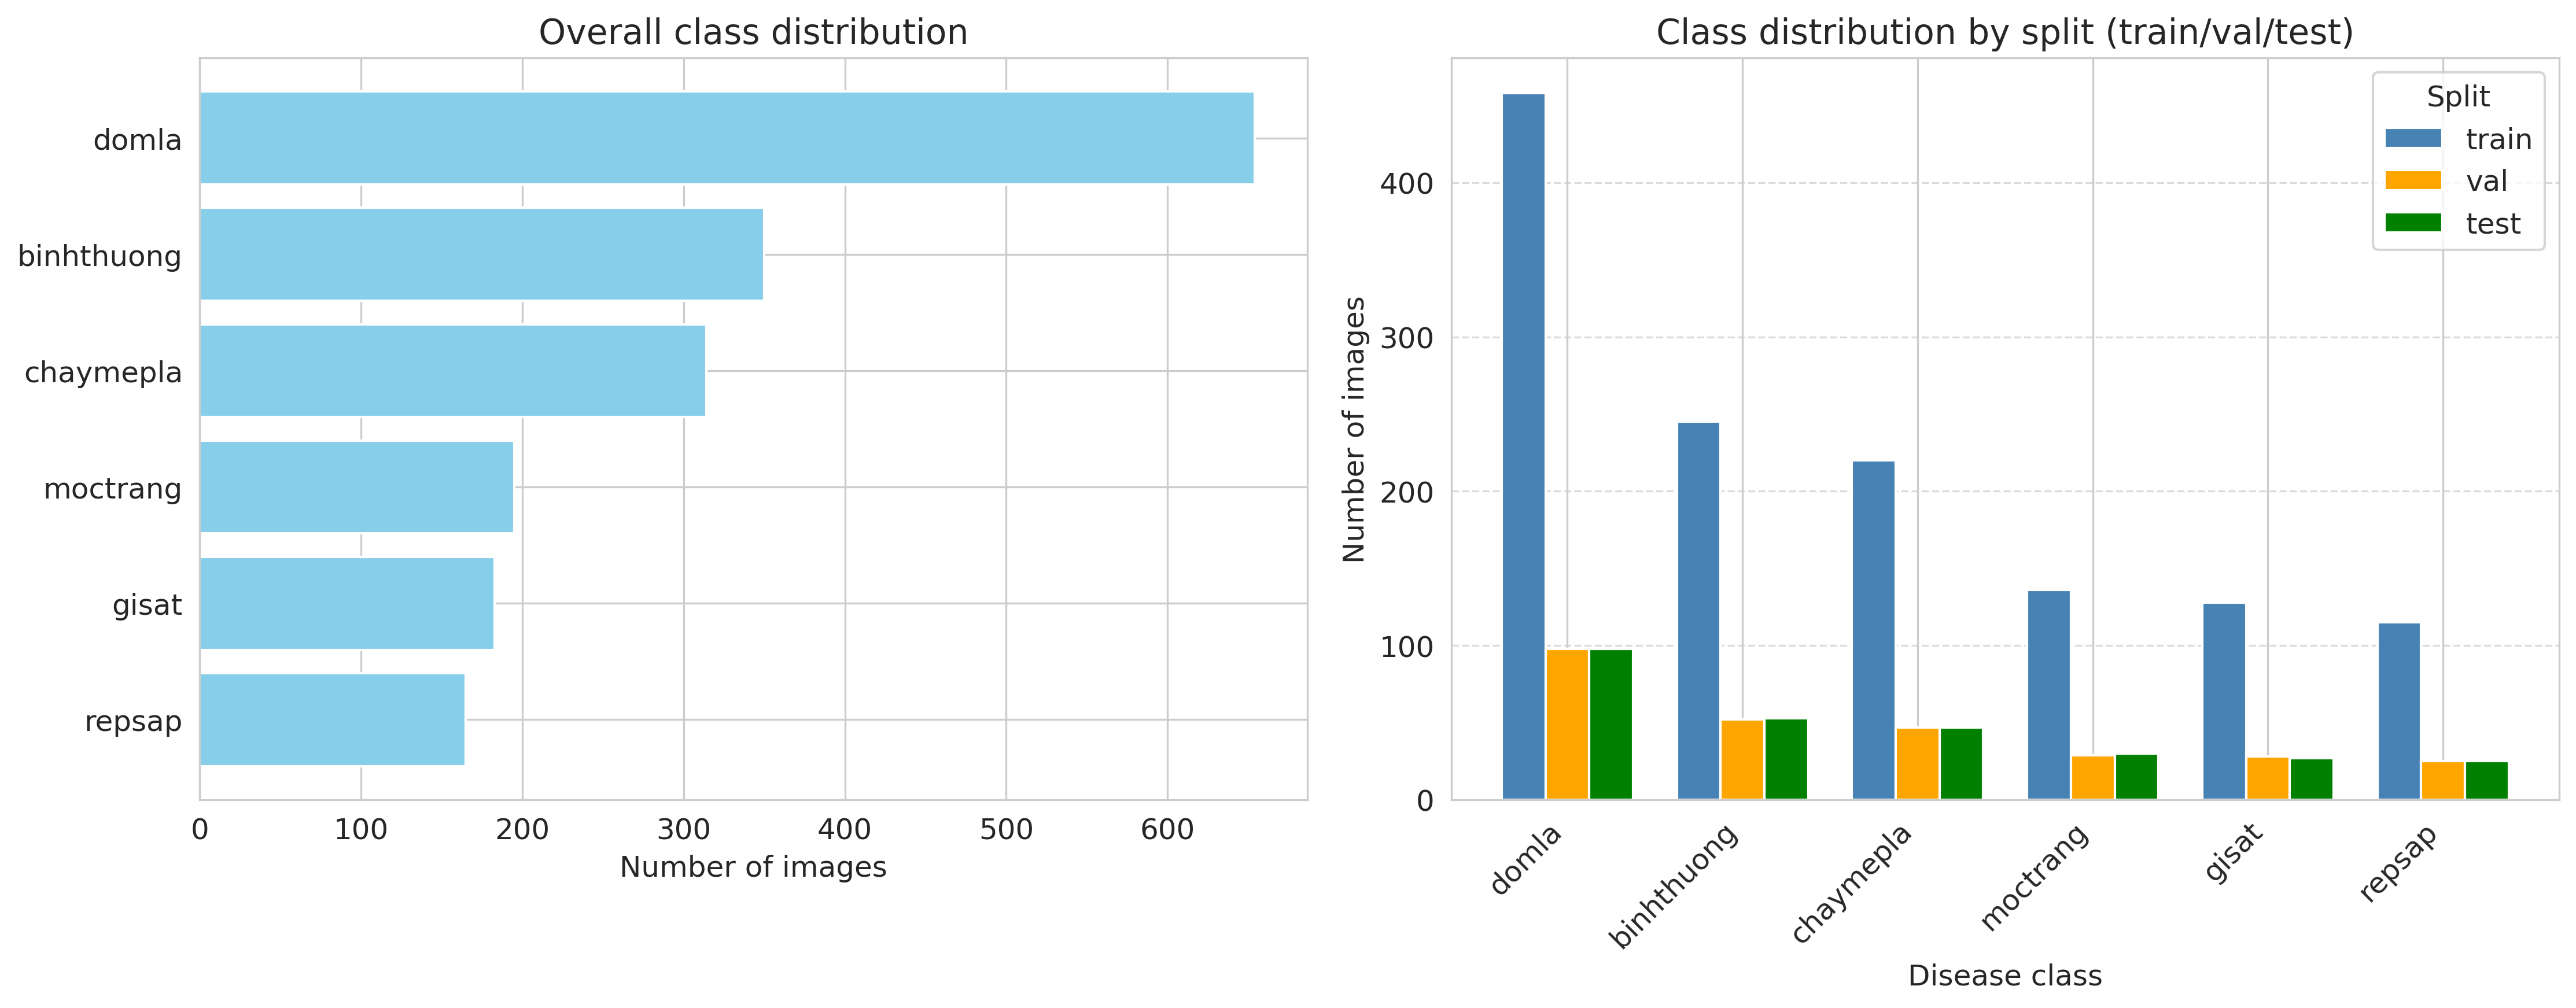
\includegraphics[width=\linewidth]{img/dataset/eda/class_distribution.png}
\caption{Class distribution. Left, overall bar chart. Right, grouped bar chart showing train/validation/test splits.}
\label{fig:class_dist}
\end{figure}


% =============================================
% Photometric Analysis
% =============================================
\subsection{Photometric Analysis}

As supporting evidence for the imaging diversity claimed in Section~\ref{sec:dataset_construction}, Figure~\ref{fig:brightness_contrast} shows that brightness varies substantially even within a single class (standard deviation 9.0 to 24.9 across classes), with \textit{domla} images alone spanning 44.4 to 153.9 and \textit{gisat} images spanning 80.5 to 182.1 on the 0-255 scale. Figure~\ref{fig:rgb_histograms} shows that classes also differ in dominant colour channel. These variations confirm that the images were collected under diverse, uncontrolled lighting and colour conditions rather than a single studio-like setup, and imply that models must be robust to such shifts rather than exploit them as shortcuts.

\begin{figure}[htbp]
\centering
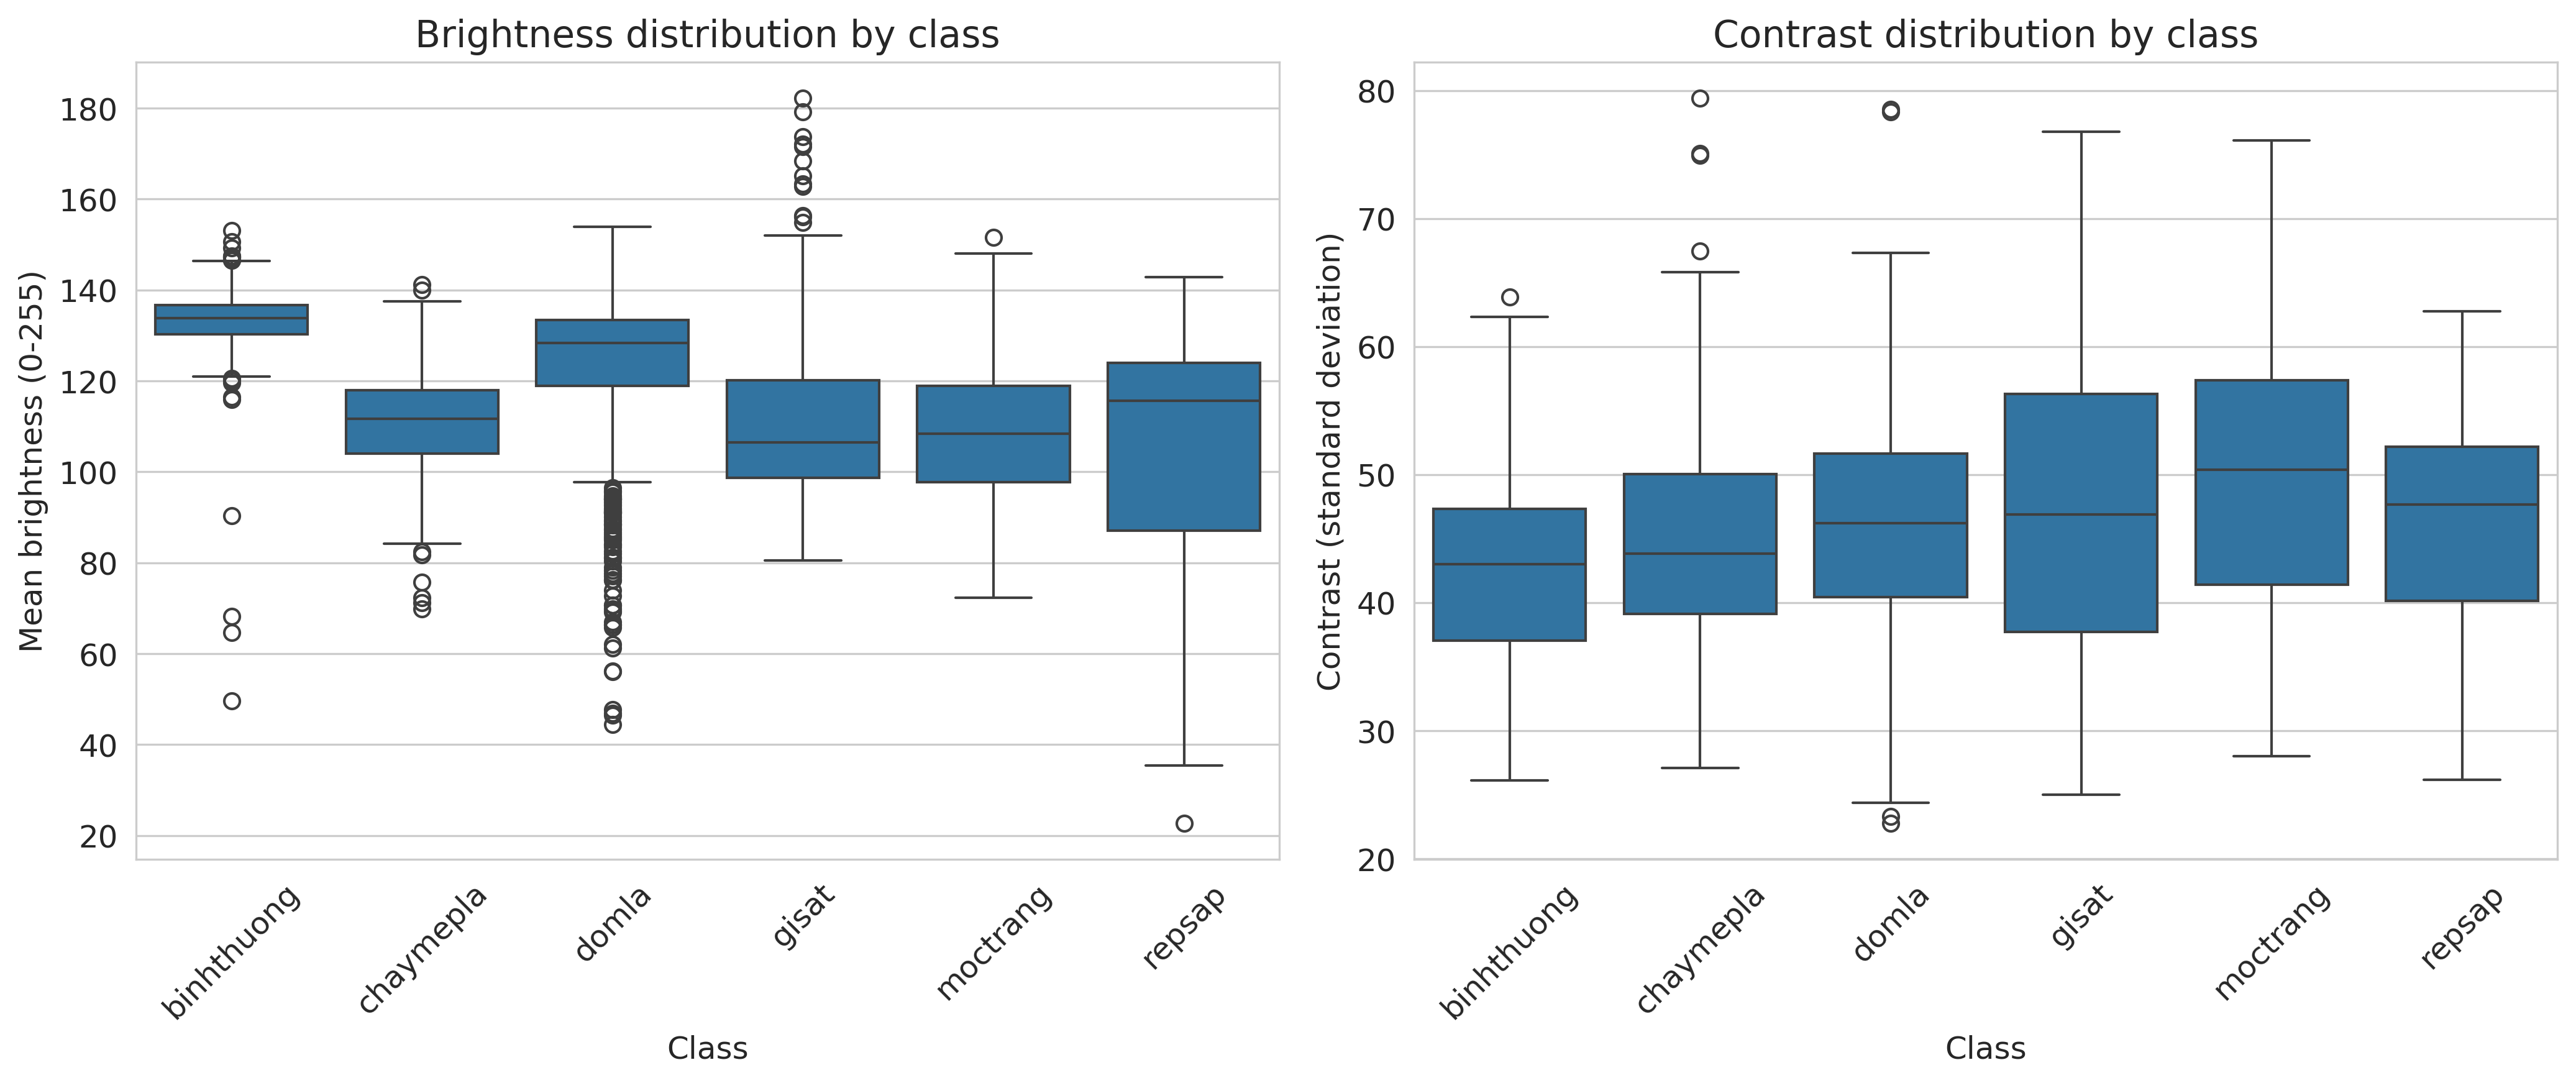
\includegraphics[width=\linewidth]{img/dataset/eda/brightness_contrast.png}
\caption{Brightness (left) and contrast (right) distributions per class.}
\label{fig:brightness_contrast}
\end{figure}

\begin{figure}[htbp]
\centering
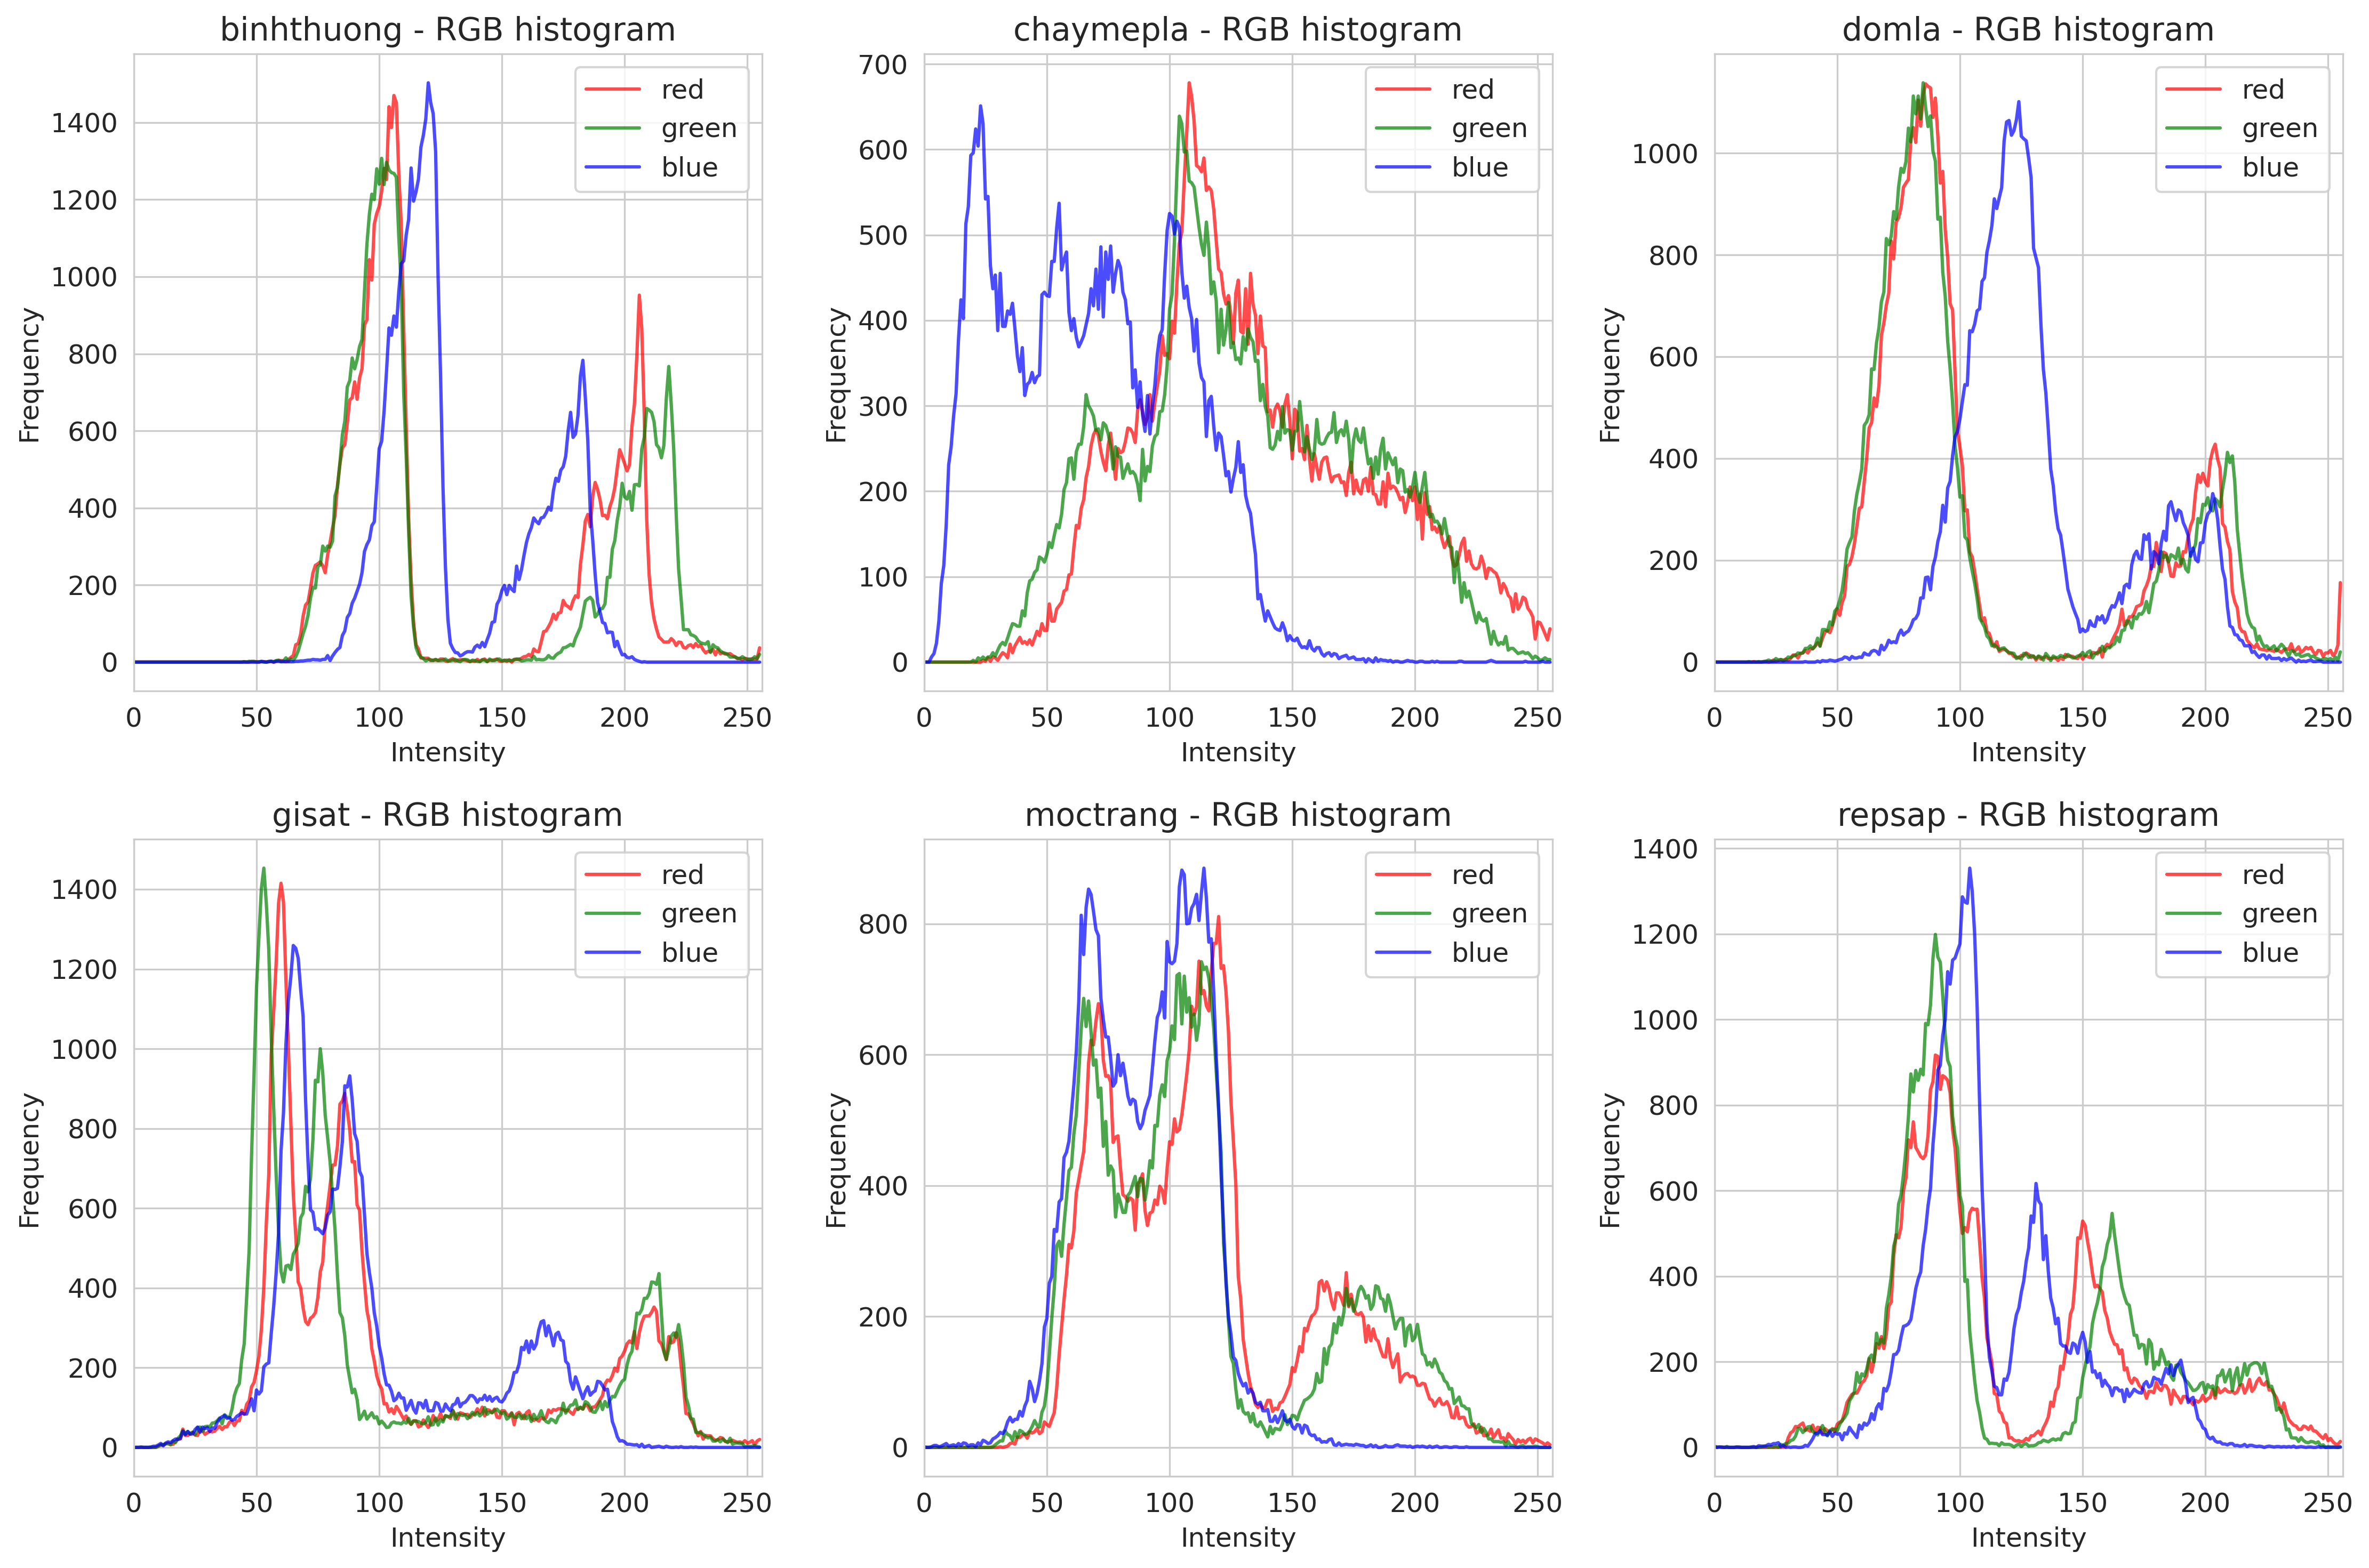
\includegraphics[width=\linewidth]{img/dataset/eda/rgb_histograms.png}
\caption{RGB histograms of one sample image per class (red, green, blue channels).}
\label{fig:rgb_histograms}
\end{figure}



% ===============================================
% Difficulty Analysis
% ===============================================
\subsection{Intrinsic Difficulty Analysis}
\label{subsec:difficulty}

To assess how challenging the dataset is for automatic classification, we performed three complementary analyses on the validation set using features extracted from a frozen ImageNet-pretrained ResNet-18 \citep{he2016deep}. The feature dimension was reduced to 512 via global average pooling.

\subsubsection{Quantitative Clustering Metrics}

We computed two standard metrics that evaluate class separability in the feature space, namely the Silhouette score \citep{rousseeuw1987silhouettes} and the Davies-Bouldin index \citep{davies1979cluster}. Table~\ref{tab:difficulty_metrics} summarises the results.

\begin{table}[htbp]
\centering
\caption{Quantitative difficulty metrics on the validation set. Lower Silhouette, higher Davies-Bouldin, and intra/inter ratio $\ge 1$ indicate strong class overlap.}
\label{tab:difficulty_metrics}
\begin{tabular}{l c}
\toprule
\textbf{Metric} & \textbf{Value} \\
\midrule
Silhouette Score & 0.0067 \\
Davies-Bouldin Index & 4.17 \\
Average intra-class distance & 12.82 \\
Average inter-class distance & 8.04 \\
Intra/Inter distance ratio & 1.59 \\
\bottomrule
\end{tabular}
\end{table}

The Silhouette score near zero indicates that samples are not closer to their own class than to neighbouring classes, implying heavy inter-class overlap. The Davies-Bouldin index (4.17) points in the same direction (lower is better separated, metric definition in \ref{app:difficulty}), though its absolute value is best read relative to other clustering configurations rather than against a fixed threshold, so it is reported here as a corroborating signal alongside Silhouette and the intra/inter distance ratio below. Notably, the intra/inter distance ratio exceeds 1 (1.59), meaning that within-class variation is larger than the separation between class centroids, a hallmark of fine-grained recognition problems.

\subsubsection{Visualisation with t-SNE}

\begin{figure}[H]
\centering
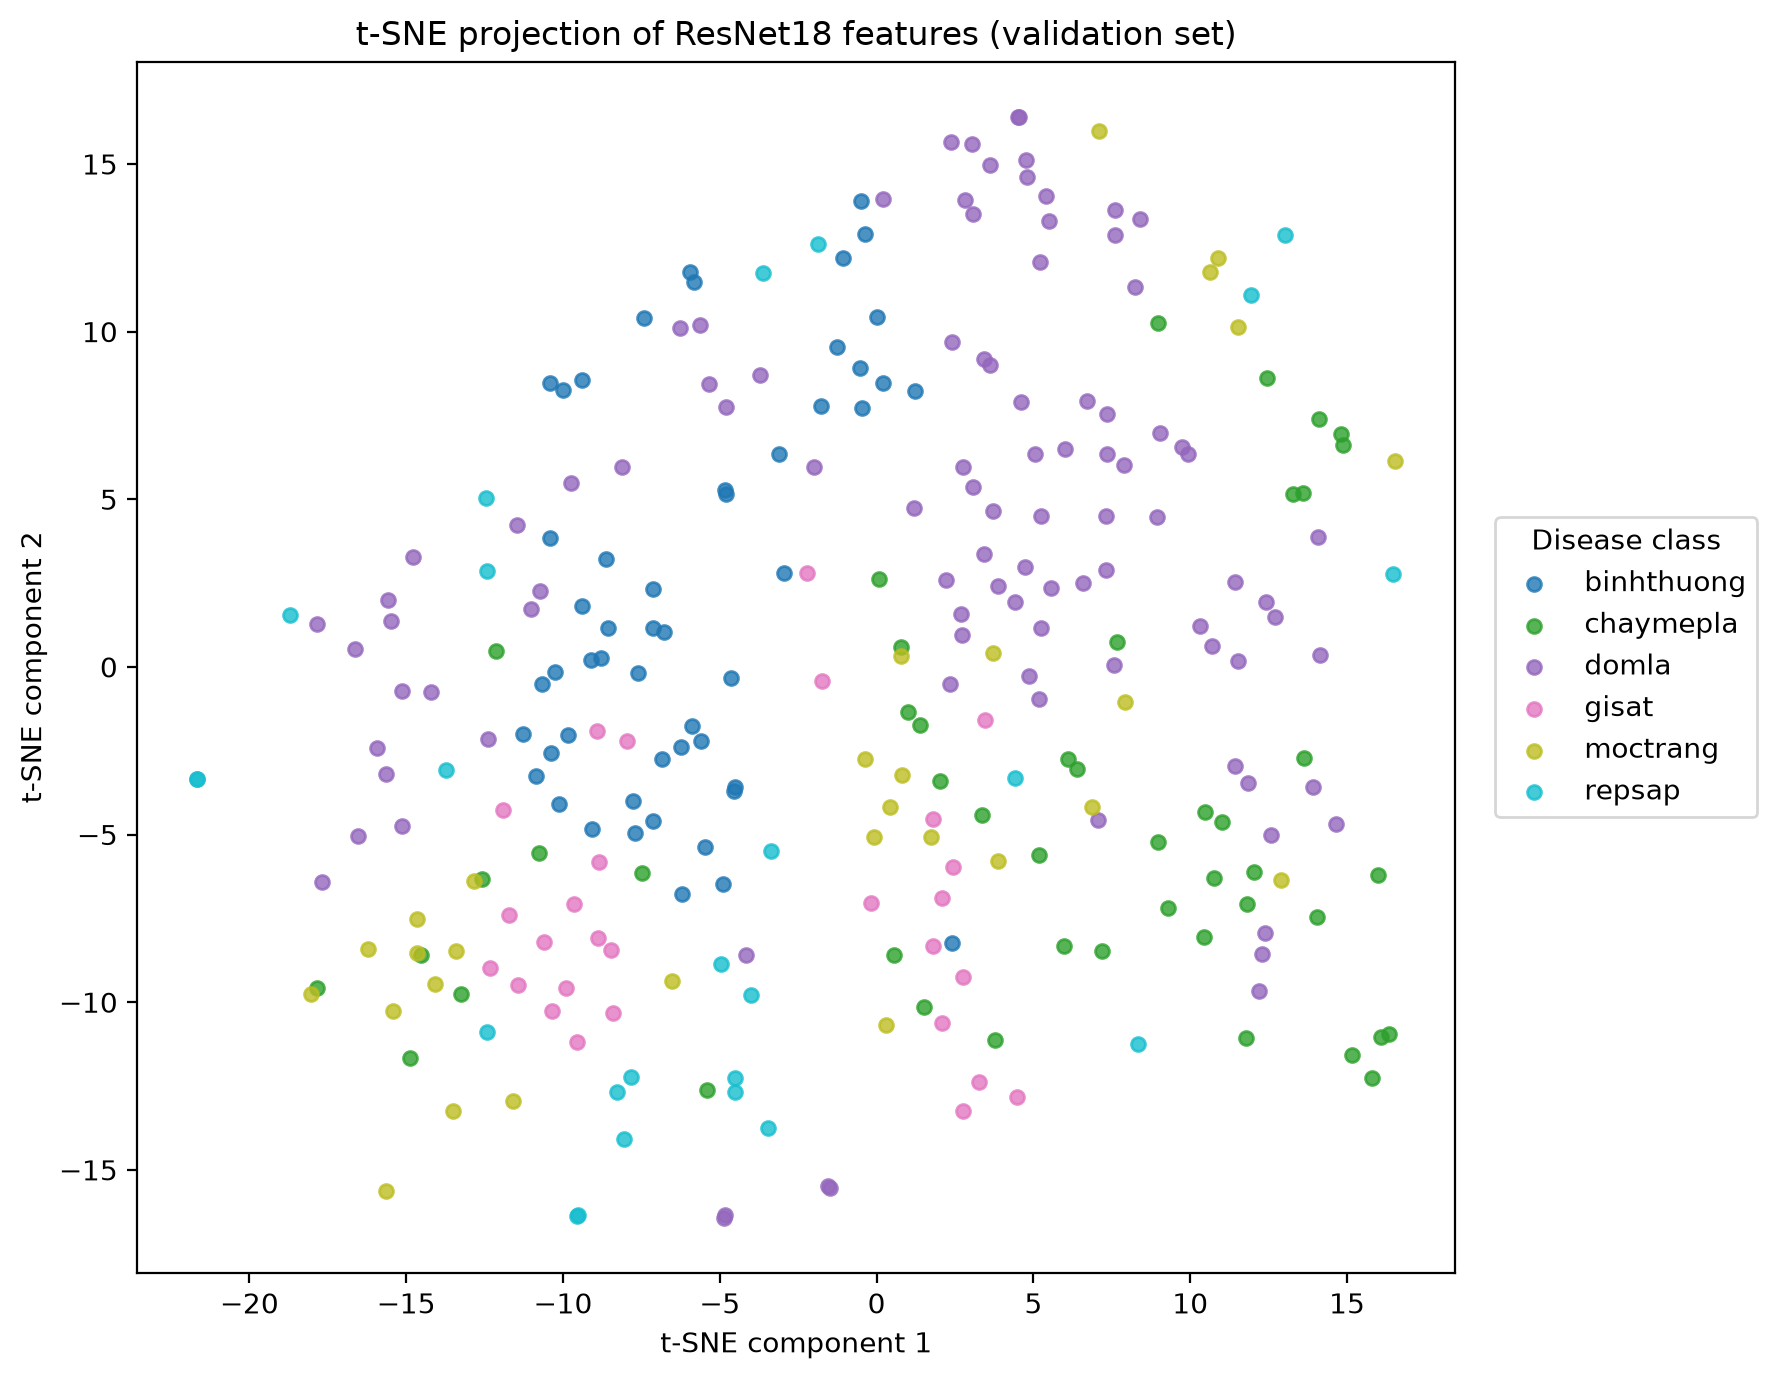
\includegraphics[width=0.8\columnwidth]{img/dataset/analysis/tsne_avocado_leaf.png}
\caption{t-SNE projection of ResNet-18 features on the validation set. Overlapping clusters confirm that disease categories are not well separated in the deep feature space.}
\label{fig:tsne}
\end{figure}

We projected the 512‑dimensional features into two dimensions using t-SNE \citep{maaten2008visualizing} with perplexity 30. Figure~\ref{fig:tsne} shows the resulting scatter plot, where each point represents a validation image and colours encode disease classes. All six classes exhibit substantial overlap without clear cluster boundaries. Classes with visually similar symptoms, such as \textit{chaymepla} (leaf scorch) and \textit{repsap} (mealybug damage), are heavily interleaved. This visual entanglement further confirms that the disease categories are not well separated in the deep feature space.

\subsubsection{Linear Separability Test}

To determine whether the frozen deep features are linearly separable by disease class, we trained a logistic regression classifier on the extracted features. Using 5‑fold cross‑validation, the model achieved a mean accuracy of \(75.25\% \pm 3.76\%\). When evaluated on a held‑out subset (30\% of the validation set, disjoint from the folds used above), the accuracy dropped to \(65.48\%\). Part of this gap is likely attributable to the small size of the validation set (279 images), which inflates the variance of both estimates. This attribution is qualitative. Unlike the architecture comparison in Section~\ref{sec:experiments} (\ref{app:bootstrap}), we did not compute a bootstrap confidence interval for the held-out estimate. The size of the reported drop should therefore be read as a point estimate whose own precision is not quantified here. Nonetheless, both figures are significantly better than random guessing (\(16.7\%\) for six classes). For comparison, Section~\ref{sec:experiments} shows that a fine-tuned, non-linear ConvNeXt-V2 model reaches \(92.14\%\) on this same AvocadoLeaf test set, a gap of roughly 17-27 percentage points over the linear probe depending on which estimate (\(75.25\%\) or \(65.48\%\)) is used. Hence, the disease classes are \textbf{not linearly separable} in the feature space, requiring non‑linear models or fine‑tuning to achieve satisfactory accuracy.

Taken together, the three analyses in this section are consistent with one another. Near-zero Silhouette, high Davies-Bouldin, and an intra/inter distance ratio above 1 all indicate substantial class overlap in feature space. The t-SNE visualisation shows this overlap directly. The linear probe confirms that this overlap cannot be resolved by a linear decision boundary. This motivates both the comparison of non-linear, fine-tuned architectures in Section~\ref{sec:experiments} and, more specifically, the use of metric-based few-shot learning in Section~\ref{subsec:fewshot}. Since frozen features are not linearly separable, a classifier trained directly on top of them generalises poorly, whereas prototypical networks learn a task-adapted embedding space in which the classes become separable.